\documentclass{article}
\usepackage[utf8]{inputenc}
\usepackage{booktabs}
\usepackage{geometry}
\usepackage{natbib}
\usepackage{graphicx}
\usepackage{float}
\usepackage{multirow}
\usepackage{subfigure}
\usepackage{listings}
\geometry{a4paper,left=2cm,right=2cm,top=2cm,bottom=2cm}
\title{Programming Assignment 2}
\author{Dong Jing 515370910182,}
\date{October 2017}



\begin{document}

\begin{titlepage}

\begin{center}


% Upper part of the page
\textsc{\LARGE }
 \\[3cm]

\textsc{\LARGE VE281}\\[5cm]

\textsc{\Large P2 REPORT}\\[5cm]


% Title
\textsc{by}\\[1cm]
\textsc{\Large Dong Jing 515370910182}\\[0.5cm]



% Bottom of the page
{\large \today}

\end{center}

\end{titlepage}
\section{Object}
I. Study the performances of linear-time selection algorithms with different input size;\\
II. Compare the results and have a better understanding about linear-time selection algorithms algorithms;\\
II. Compare the runtime of two selection algorithms and the runtime of the selection algorithms with the sorting algorithms;\\
\section{Design}
Note: all program are executed on Ubuntu (64-bit) with memory equal to 2048 MB on Oracle VM VirtualBox 5.1.22 r115126.\\
\\
Use mrand48() to generate random arrays. And use rand()\%$n$ to generate the order number less than $n$. For a given input size, to avoid the influence of the specified order $i$, I test different order $i$ according to the size of the array. Besides, I also use quick sorting with in place to sort the array and get the value of the order $i$. Comparing the runtime, I can find the efficiency of the selecting algorithm.\\
For the size of array, I choose $n$ equal to 10, 50, 100, 500, 1000, 5000, 10000, 50000, 100000, 500000 and 1000000. For different size of array, I choose different times of the order $i$ to test the runtime efficiency.
When $n=10$, test 5 different orders. When $n=50$, test 10 different orders. When $n=100$, test 20 different  orders. When $n=500$, test 50 different orders. When $n=1000$, test 50 different orders. When $n=5000$, test 100 different orders. When $n=10000$, test 500 different orders. When $n=50000, 100000, 500000,1000000$, choose 1000 different orders to see the runtime efficiency of two linear-time selection algorithms.\\
\section{Result}
Table 1 shows are data we recorded. The unit of all data is CLOCK\_PER\_SEC.\\
\begin{table}[!hbp]
\centering
\begin{tabular}{|c||c|c|c|}
\hline
Input Size & Random selection & Deterministic selection & Quick sorting selection\\
\hline
10 & 12 & 1 & 15 \\
50 & 16 & 2 & 58 \\
100 & 27 & 6 & 113\\
500 & 30 & 42 & 983\\
1000 & 44 & 108 & 1888\\
5000 & 171 & 1076 & 7908\\
10000 & 232 & 1022 & 13479\\
50000 & 1510 & 6207 & 109161\\
100000 & 3420 & 13719 & 269834\\
500000 & 13969 & 57528 & 989549\\
1000000 & 25049 & 93762 & 1163245\\
\hline
\end{tabular}
\caption{Runtime efficiency comparison between two selection algorithms and quick sorting selection algorithm.}
\end{table}
Then, use Matlab to plot three curves representing the runtime efficiency on different input size of three algorithms. \\
\begin{figure}[H]
\centering
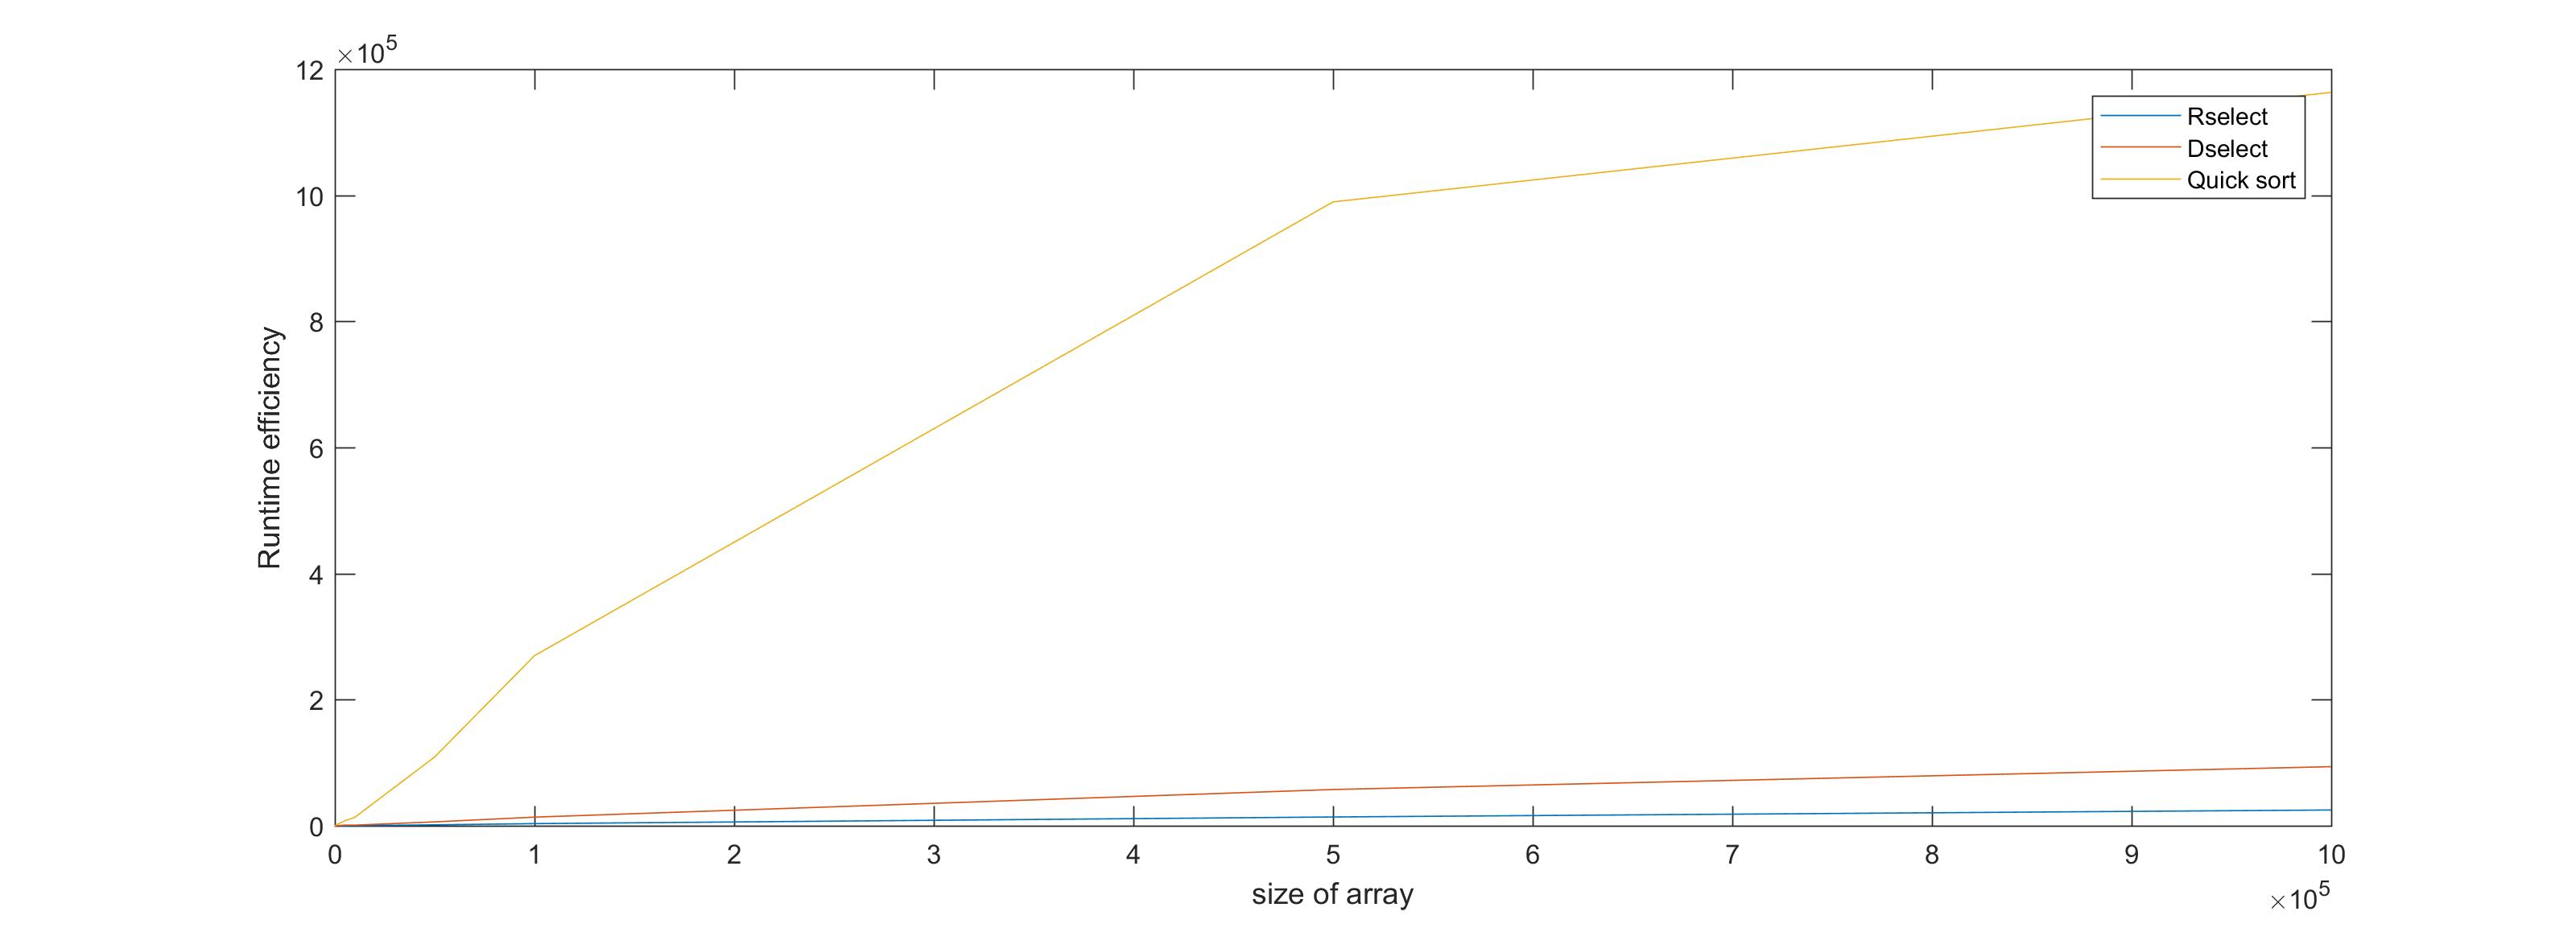
\includegraphics[width=\textwidth]{1.jpg}
\caption{Comparison of runtime efficiency.}
\end{figure}
\begin{figure}[H]
\centering
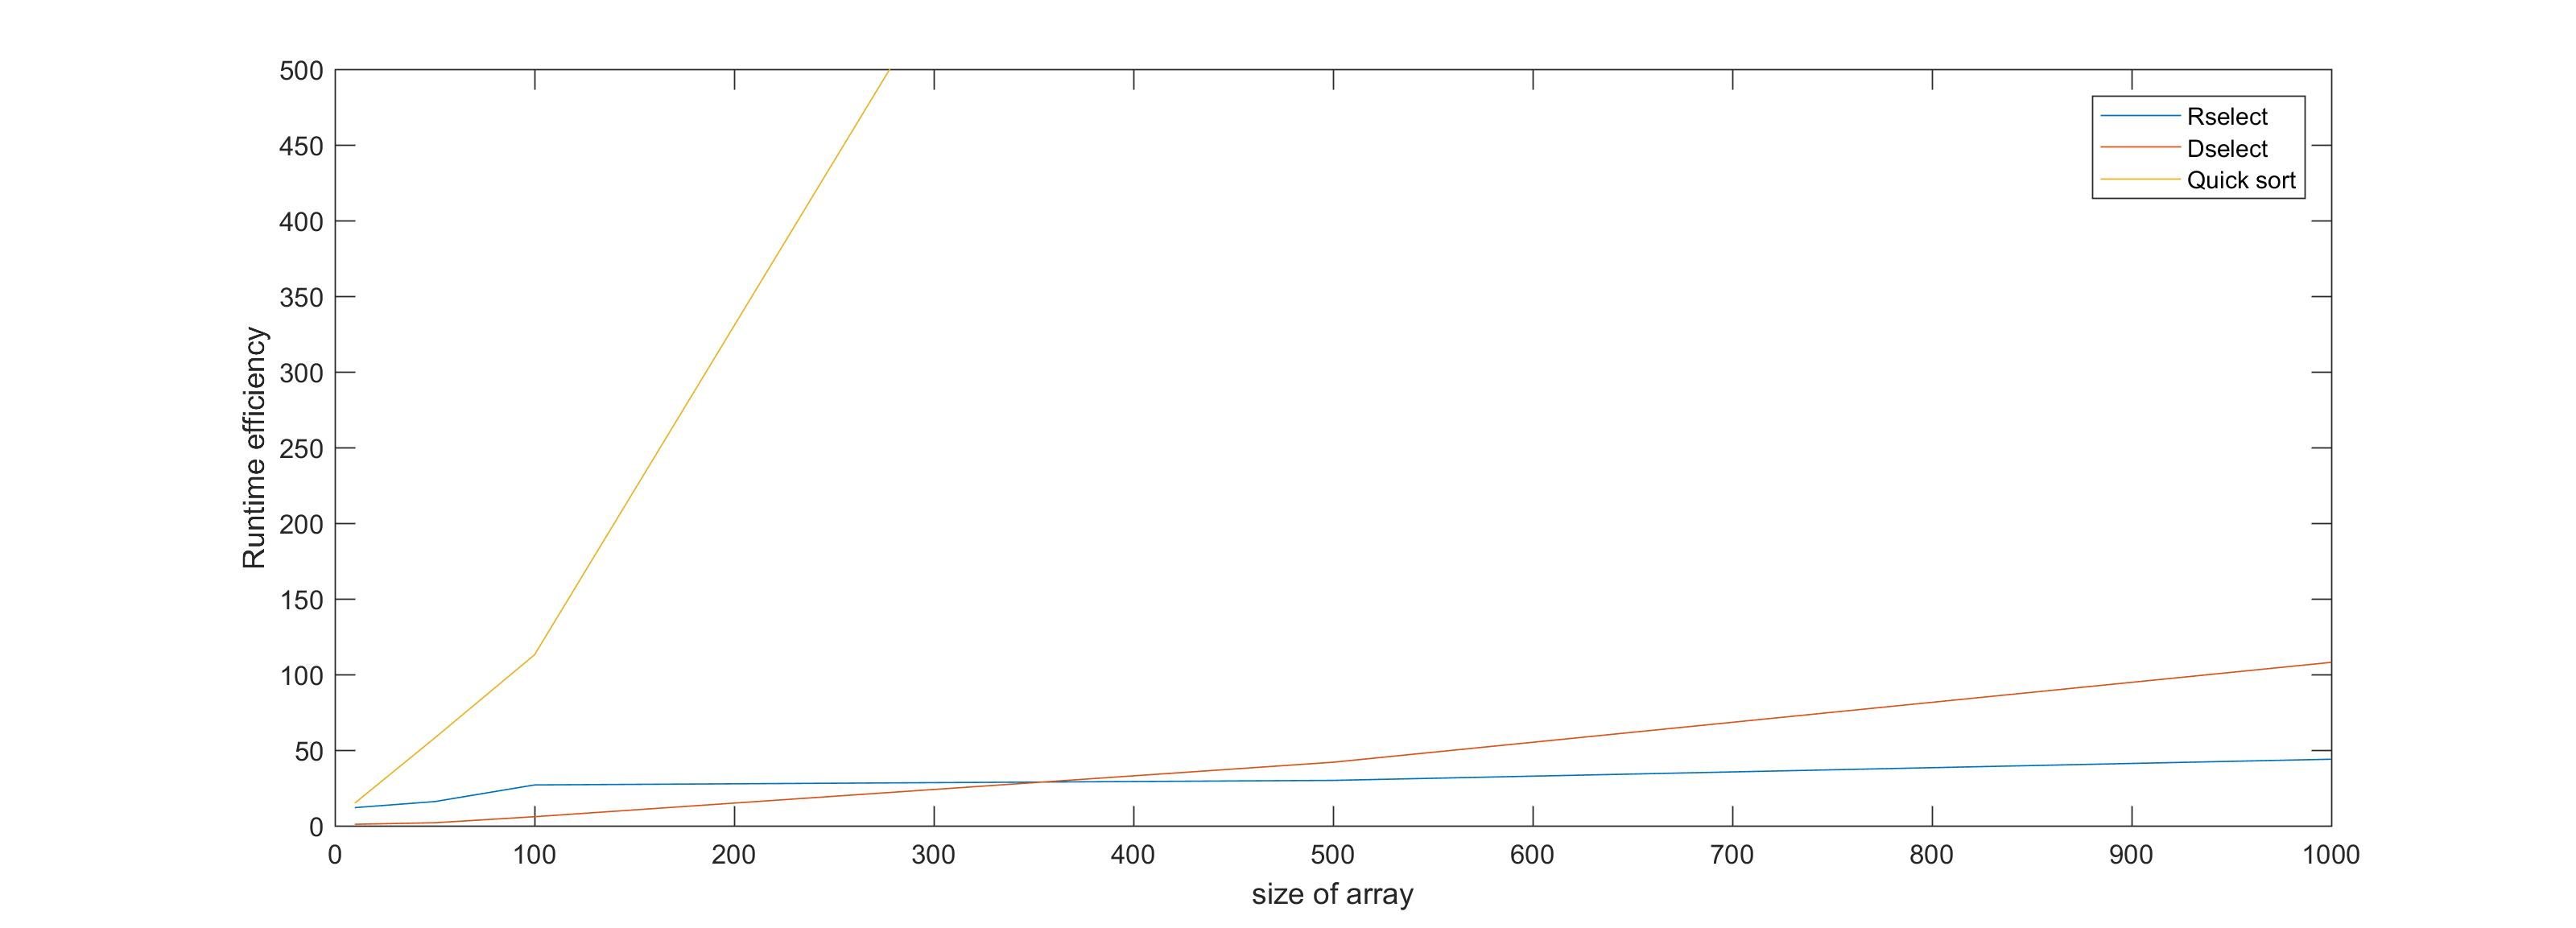
\includegraphics[width=\textwidth]{2.jpg}
\caption{Comparison of runtime efficiency on small input size.}
\end{figure}
\begin{figure}[H]
\centering
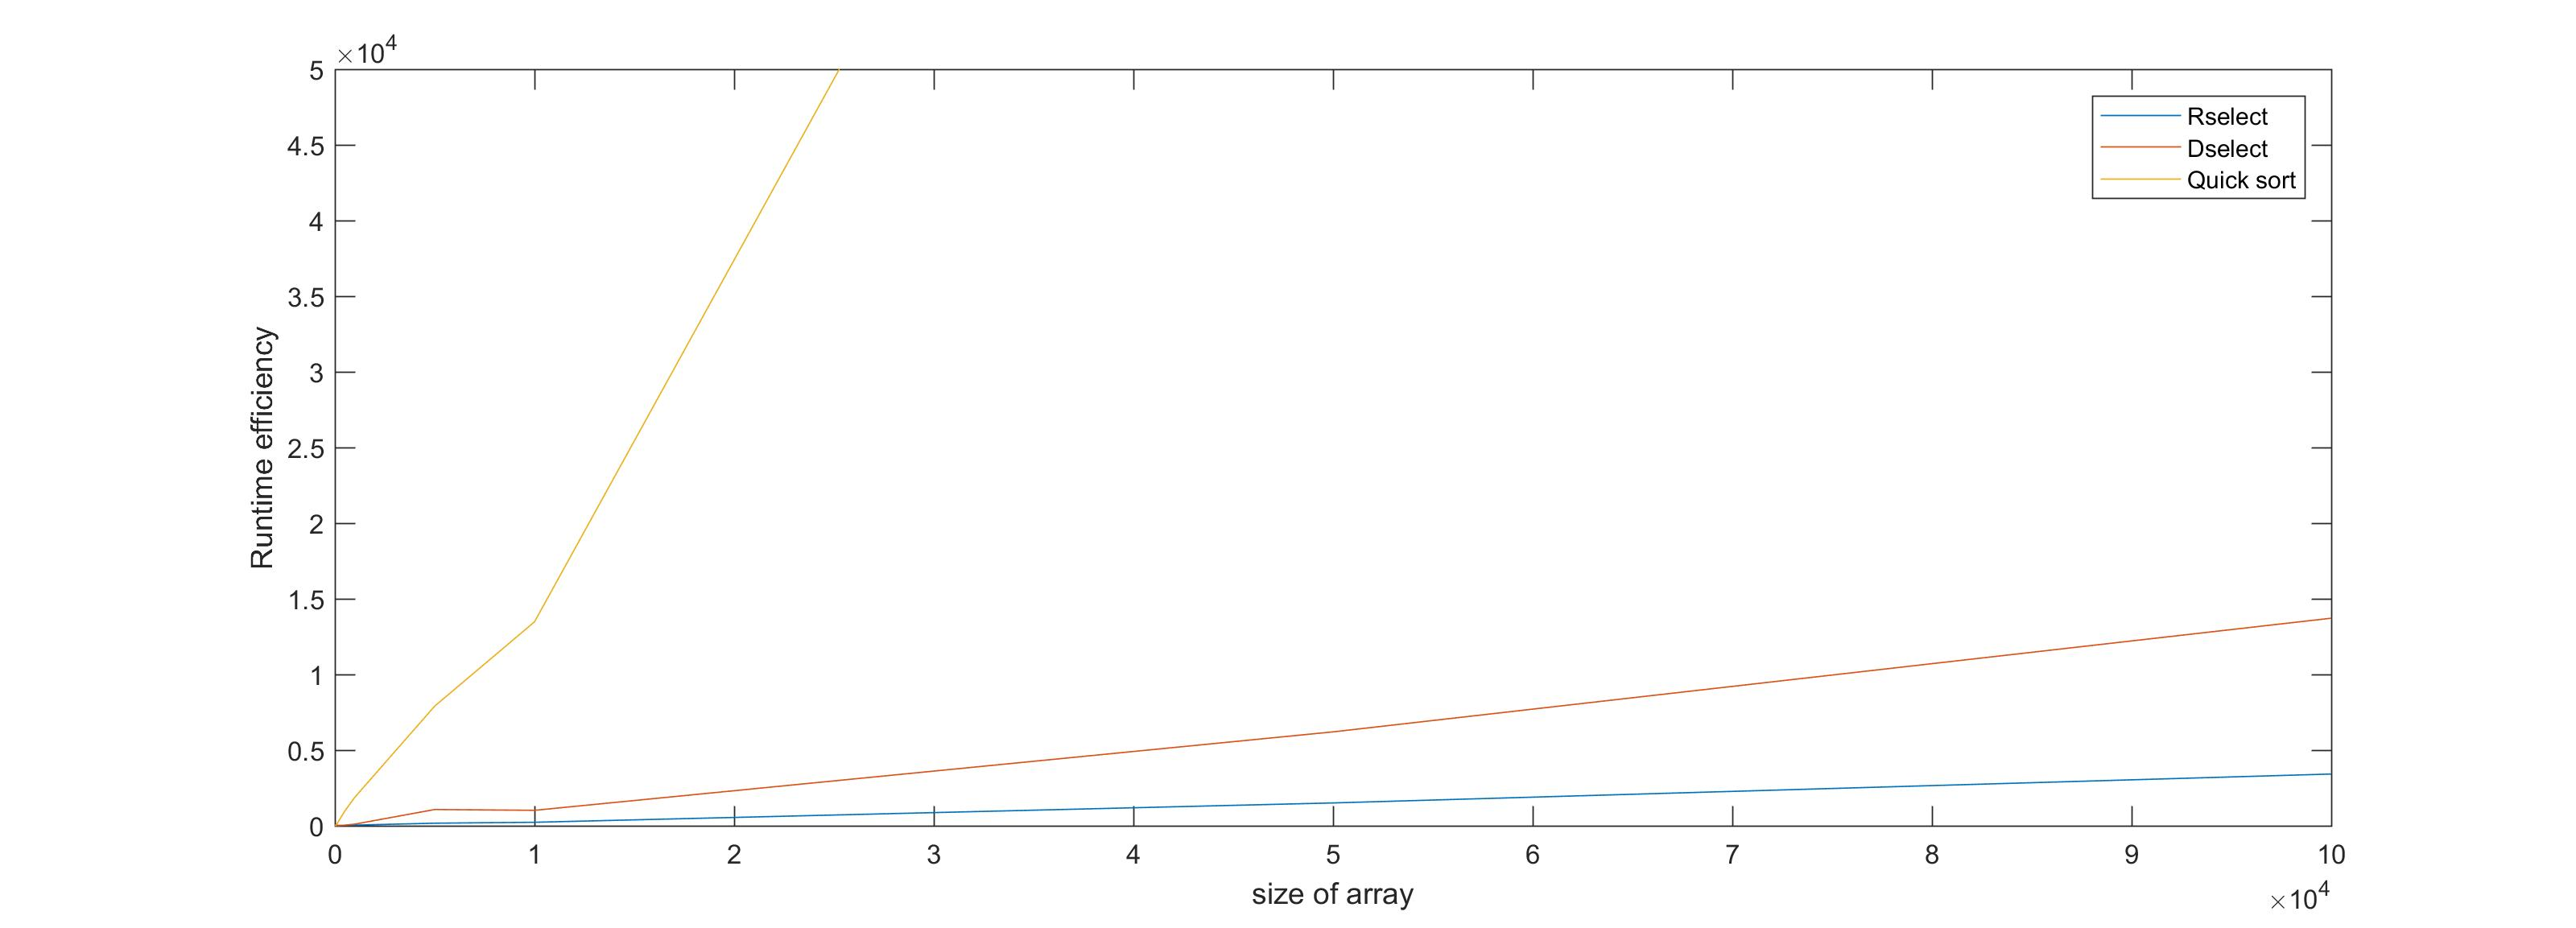
\includegraphics[width=\textwidth]{3.jpg}
\caption{Comparison of runtime efficiency on middle input size.}
\end{figure}
In all three figures, blue curve represents the runtime efficiency of random selection algorithm. Orange curve shows the relationship between the runtime efficiency of deterministic selection algorithm and the input size. Yellow curve is the runtime efficiency of the quick sorting selection algorithm. \\
As we can see, figure 1 shows the comparison of three curves from the input size equal to 10 to the input size equal to 1000000. It is obvious that two linear-time selection algorithms are faster than the quick sorting selection algorithm a lot, even quick sorting algorithm is a fast sorting algorithm. And we find that random selection algorithm is a little faster than the deterministic selection algorithm. And we find both two curves of selection algorithms are linear, which shows the runtime of two selection algorithms is proportional to the size of array. It may be the reason why they are called linear-time selection algorithms.\\
In the figure 2, we can see even for the small input size, quick sorting selection algorithm is much slower than two linear-time selection algorithms. And for the small input size like 10 or 50, deterministic selection algorithm is faster than random selection algorithm. But the slope of the line of deterministic selection algorithm is greater than the slope of the line of random selection algorithm, which leads to the result that for the large input size, random selection algorithm is faster than the deterministic selection algorithm. \\
In figure 3, we can find as the input size grows, the efficiency of random selection algorithm is more obvious. And two curves of two linear-time selection algorithms are more like two lines in this figure. Because they are linear, we can easily estimate the runtime if we need to use the selection algorithm to the larger input size. \\
\section{Discussion and Conclusion}
From three figures, we can know that two linear-time selection algorithms is faster than the quick sorting selection algorithm. This is why we want to use selection algorithms if we only need to know the value of some order in an array. It can save lots of time. And we find, if the size of array is large enough, random selection algorithm is faster than the deterministic selection algorithm, which advice us to use random selection algorithm for some large input size like 1000. Besides, we find the curves of two linear-time selection algorithms are like lines, which shows why they are called linear-time selection algorithms. \\
\\
There may be some errors for large input size. Because my computer is not good enough, I only test a few orders for large input size, which may be considered too few compared to the size of array. But I think it is enough. Even we test more different orders the result of two selection algorithms is still linear. And I do not generate lots of different array of same size to test the runtime efficiency because I think what matter more in this test is the specified order $i$. But it may lead to the wrong result of quick sorting selection algorithm because we already know that different distribution of numbers will lead to different runtime of quick sorting algorithm. I think this difference between different array is too small compared to the large difference between two linear-time selection algorithms and quick sorting selection algorithm.\\
\\
In conclusion, in this programming project, I try to program two linear-time selection algorithms by myself, which helps me understand them better. I clearly know how these two algorithms works and what is the difference between them. I also see the efficiency of the linear-time selection algorithms. They looks like quick sorting algorithm but they are much more faster. They just use some similar idea from the quick sorting algorithm. \\
\section{Appendix}
time.cpp\\
\#include $<$iostream$>$\\
\#include $<$fstream$>$\\
\#include $<$sstream$>$\\
\#include $<$string$>$\\
\#include $<$cstdlib$>$\\
\#include $<$climits$>$\\
\#include $<$ctime$>$\\
\#include $<$cassert$>$\\
\#include "selection.h"\\
\#include "sort.h"\\
\\
using namespace std;\\
\\
int main()\\
\{\\
    srand((unsigned)time(NULL));\\
    int n,i,r,k,km;\\
    n=10;\\
    clock\_t t[3];\\
    clock\_t tem;\\
    r=0;\\
    while (n$<=$1000000)\\
    \{\\
	long int *a0,*a1,*a2,*a3;\\
	a0=new long int [n];\\
	a1=new long int [n];\\
	a2=new long int [n];\\
    a3=new long int [n];\\
	for (int j=0;j$<$n;j++) \{a0[j]=mrand48();a1[j]=a0[j];a2[j]=a0[j];a3[j]=a0[j];\}\\
	k=0;\\
	switch (n)\\
	\{\\
	    case 10: km=5;break;\\
	    case 50: km=10;break;\\
	    case 100: km=20;break;\\
	    case 500: km=50;break;\\
	    case 1000: km=50;break;\\
	    case 5000: km=100;break;\\
	    case 10000: km=500;break;\\
	    case 50000: km=1000;break;\\
	    case 100000: km=1000;break;\\
	    case 500000: km=1000;break;\\
	    case 1000000: km=1000;break;\\
	\}\\
	while (k$<$km)\\
	\{\\
	    i=rand()\%n;\\
	    tem=clock();\\
	    Rselect(a0,n,i);\\
	    tem=clock()-tem;\\
	    t[0]=(k*t[0]+tem)/(k+1);\\
	    tem=clock();\\
	    Dselect(a1,n,i);\\
	    tem=clock()-tem;\\
	    t[1]=(k*t[1]+tem)/(k+1);\\
	    k++;\\
        for (int j=0;j$<$n;j++)\{a0[j]=a3[j];a1[j]=a3[j];\}\\
	\}\\
    tem=clock()\\
    quick\_inplace(a,0,n-1);\\
    t[2]=clock()-tem;
	cout$<<$endl$<<$"Input size is "$<<$n$<<$endl;\\
	cout$<<$"Rselect:\t"$<<$t[0]$<<$endl;\\
	cout$<<$"Dselect:\t"$<<$t[1]$<<$endl;\\
	cout$<<$"Quicksort\t"$<<$t[2]$<<$endl;\\
	if (r\%2==0) n=n*5;\\
	else n=n*2;\\
	r++;\\
	delete [] a0;\\
	delete [] a1;\\
	delete [] a2;\\
    delete [] a3;\\
    \}\\
\}\\
\\
selection.h\\
\#ifndef \_\_SELECTION\_H\_\_\\
\#define \_\_SELECTION\_H\_\_\\
\\
long int Rselect(long int *a, int n, int i);\\
\\
int partition(long int *a, int n,int p);\\
\\
long int Dselect(long int *a, int n, int i);\\
\\
long int median(long int *a, int n);\\
\\
\#endif // \_\_SELECTION\_H\_\_\\
\\
selection.cpp\\
\#include $<$iostream$>$\\
\#include $<$fstream$>$\\
\#include $<$sstream$>$\\
\#include $<$string$>$\\
\#include $<$cstdlib$>$\\
\#include $<$climits$>$\\
\#include $<$ctime$>$\\
\#include $<$cassert$>$\\
\#include "selection.h"\\
\\
using namespace std;\\
\\
long int Rselect(long int *a, int n, int i)\\
\{\\
    srand((unsigned)time(NULL));\\
    int p=rand()\%(n);\\
    int j=partition(a,n,p);\\
    if (j==i) return a[j];\\
    if (j$>$i) return Rselect(a, j, i);\\
    else return Rselect(a+j+1,n-j-1,i-j-1);\\
\}\\
\\
int partition(long int *a, int n, int p)\\
\{\\
    int i=1;\\
    int j=n-1;\\
    long int tem;\\
    tem=a[p];\\
    a[p]=a[0];\\
    a[0]=tem;\\
    if (i==j)\\
    \{\\
        if (a[0]$>$a[1]) {tem=a[1];a[1]=a[0];a[0]=tem;}\\
        else j--;\\
    \}\\
    else while (i$<$j)\\
        \{\\
            while ((i$<$n-1)\&\&(a[i]$<$a[0])) i++;\\
            while ((j$>$0)\&\&(a[j]$>$=a[0])) j--;\\
            if (i$<$j) \{tem=a[i];a[i]=a[j];a[j]=tem;\}\\
            else \{tem=a[j];a[j]=a[0];a[0]=tem;\}\\
        \}\\
    return j;\\
\}\\
\\
long int Dselect(long int *a, int n, int i)\\
\{\\
    if (n==1) return a[0];\\
    else\\
    \{\\
        long int C[(n-1)/5+1];\\
	    int C1[(n-1)/5+1];\\
        int k=0, j=0;\\
        for (k;k$<$(n-1)/5;k++)\\
            \{\\C[k]=median(\&a[k*5],5);\}\\
        C[k]=median(\&a[k*5],n-5*k);\\
        long int p=Dselect(\&C[0],(n-1)/5+1,n/10);\\
	int p1;\\
	for (int m=0;m<n;m++)\\
	if (a[m]==p) \{\\p1=m;break;\}\\
        j=partition(a,n,p1);\\
        if (j==i) return a[j];\\
        if (j$>$i) return Dselect(a, j, i);\\
        else return Dselect(a+j+1,n-j-1,i-j-1);\\
    \}\\
\}\\
\\
long int median(long int *a, int n)\\
\{\\
    int j;\\
    long int tem;\\
    for (int i=1;i$<$n;i++)\\
    \{\\
        tem=a[i];\\
        j=i-1;\\
        while ((j$>$-1)\&\&(tem$<$a[j]))\\
        \{\\
            a[j+1]=a[j];\\
            j--;\\
        \}\\
        a[j+1]=tem;\\
    \}\\
    return a[(n-1)/2];\\
\}\\
\\
sort.h\\
\#ifndef \_\_SORT\_H\_\_\\
\#define \_\_SORT\_H\_\_\\
\\
void quick\_inplace(long int *a, int left, int right);\\
\\
int partition\_in(long int *a, int left, int right);\\
\\
\#endif // \_\_SORT\_H\_\_\\
\\
sort.cpp\\
\#include $<$iostream$>$\\
\#include $<$fstream$>$\\
\#include $<$sstream$>$\\
\#include $<$string$>$\\
\#include $<$cstdlib$>$\\
\#include $<$climits$>$\\
\#include $<$ctime$>$\\
\#include $<$cassert$>$\\
\#include "sort.h"\\
\\
using namespace std;\\
\\
void quick\_inplace(long int *a, int left, int right)\\
\{\\
    int pivotat;\\
    if (left$>$=right) return;\\
    pivotat=partition\_in(a,left,right);\\
    quick\_inplace(a,left,pivotat-1);\\
    quick\_inplace(a,pivotat+1,right);\\
\}\\
\\
int partition\_in(long int *a, int left, int right)\\
\{\\
    srand((unsigned)time(NULL));\\
    int i=left+1, j=right;\\
    int p=rand()\%(right-left+1)+left;\\
    long int tem;\\
    tem=a[p];\\
    a[p]=a[left];\\
    a[left]=tem;\\
    if (i==j)\\
    \{\\
	if (a[left]$>$a[right])\\
	\{\\
	    tem=a[left];\\
	    a[left]=a[right];\\
	    a[right]=tem;\\
	\}\\
	else j--;\\
    \}\\
    else while (i$<$j)\\
    \{\\
        while ((i$<$right)\&\&(a[i]$<$a[left])) i++;\\
        while ((j$>$left)\&\&(a[j]$>$=a[left])) j--;\\
        if (i$<$j) \{tem=a[i];a[i]=a[j];a[j]=tem;\}\\
        else \{tem=a[j];a[j]=a[left];a[left]=tem;\}\\
    \}\\
    return j;\\
\}\\
\\
\end{document}
